\documentclass[12pt, letterpaper]{extarticle}

\usepackage{geometry}
\usepackage{graphicx}
\usepackage{setspace}
\usepackage[T1]{fontenc}
\usepackage{lmodern}
\usepackage{amsmath}
\usepackage{amssymb}
\usepackage[spanish]{babel}
\usepackage{csquotes}
\usepackage[hidelinks]{hyperref}
\usepackage[shortlabels]{enumitem}
\usepackage{mathtools}
\usepackage{array}
\usepackage{subfiles}

\geometry{left=1in, bottom=1in, right=1in, top=1in}

\newcommand{\newSection}[1]{\section*{#1}\addcontentsline{toc}{section}{#1}}
\newcommand{\newSubSection}[1]{\subsection*{#1}\addcontentsline{toc}{subsection}{#1}}
\newcommand{\newSubSubSection}[1]{\subsubsection*{#1}\addcontentsline{toc}{subsubsection}{#1}}
\newcommand{\unit}[1]{\ensuremath{\; \mathrm{#1}}}

\begin{document}

\subfile{Portada.tex}

\newpage

\tableofcontents

\newpage

\newSection{Aplicaciones de los amplificadores operacionales}

\newSubSection{Amplificador restador inversor}

\begin{figure}[h]
    \centering
    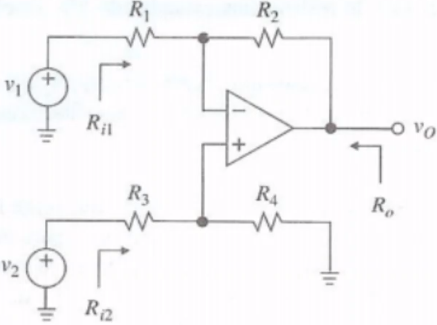
\includegraphics[width=0.5\textwidth]{Media/amplificador_restador_inverso.png}
    \caption{Amplificador restador inversor.}
    \label{Fig: Amplificador restador inversor}
\end{figure}

\begin{equation*}
    V_{out} = V_{2}\left(\frac{(R_{1}+R_{2})R_{4}}{(R_{4}+R_{3})R_{1}}\right)
             -V_{1}\left(\frac{R_{2}}{R_{1}}\right)
\end{equation*}

En el caso de que $R_{1}=R_{2}=R_{3}=R_{4}=R$:
\begin{equation*}
    V_{out} = V_{2} - V_{1}
\end{equation*}

\newSubSection{Amplificador diferenciador (derivador) inversor}

\begin{figure}[h]
    \centering
    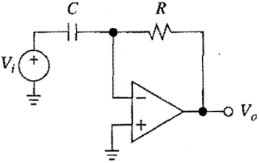
\includegraphics[width=0.5\textwidth]{Media/amplificador_diferenciador.png}
    \caption{Amplificador diferenciador}
    \label{Fig: Amplificador diferenciador}
\end{figure}

\begin{equation*}
    V_{out} = -RC\left(\frac{dV_{in}(t)}{dt}\right)
\end{equation*}


\newSubSection{Amplificador integrador inversor}

\begin{figure}[h]
    \centering
    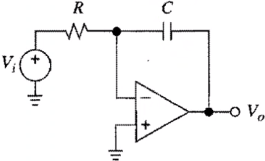
\includegraphics[width=0.5\textwidth]{Media/amplificador_integrador.png}
    \caption{Amplificador integrador}
    \label{Fig: Amplificador integrador}
\end{figure}

\begin{equation*}
    V_{out} = -\frac{1}{RC}\int V_{in}(t) \; dt
\end{equation*}

\end{document}